\documentclass[a4j,11pt]{jarticle}
\usepackage{fancybox}
\usepackage{mathptmx}
\usepackage{ascmac}
\usepackage{amsmath}
%\usepackage[top=30truemm,bottom=30truemm,left=25truemm,right=25truemm]{geometry}
\usepackage{algorithm}
\usepackage{algorithmic}
\usepackage{bm}
\usepackage[dvipdfmx]{graphicx}
\usepackage[dvipdfmx]{color}
\usepackage{subcaption}
\usepackage{here}
\usepackage{wrapfig}
\bibliographystyle{apalike}
%\setlength{\voffset}{-25.4mm}
\setlength{\topmargin}{-17.5mm}   %トップとヘッダの間隔
%\setlength{\headheight}{20mm}   %ヘッダの高さ
%\setlength{\headsep}{0mm}   %ヘッダとテキストの間隔
\setlength{\textwidth}{45zw}   %テキストの幅
\setlength{\hoffset}{-10mm}
\setlength{\textheight}{45\baselineskip}   %テキストの高さ
%\addtolength{\textheight}{\topskip}
%\setlength{\footskip}{0mm}
%\setlength{\oddsidemargin}{21.5mm}   %サイドとテキストの間隔(奇数ページ)
%\setlength{\evensidemargin}{21.5mm}   %サイドとテキストの間隔(偶数ページ)
\pagestyle{empty}   %ページ番号なし
\newcommand{\g}[1]{\boldsymbol{#1}}
\newcommand{\lw}[1]{\smash{\lower2.0ex\hbox{#1}}}
\renewcommand{\baselinestretch}{1.0}
\setlength\floatsep{0pt}
\setlength\textfloatsep{0pt}
\setlength\intextsep{0pt}
\setlength\abovecaptionskip{0pt}
\makeatletter
\def\theequation{\arabic{equation}}   %数式番号を(章.式)形式
\@addtoreset{equation}{section}
%\def\thefigure{\thesection.\arabic{figure}}   %図番号を(章.図)形式
%\@addtoreset{figure}{section}
%\def\thetable{\thesection.\arabic{table}}   %表番号を(章.表)形式
%\@addtoreset{table}{section}
\def\tr{\mathop{\operator@font tr}\nolimits}
\def\grad{\mathop{\operator@font grad}\nolimits}
\def\St{\mathop{\operator@font St}\nolimits}
\def\Hess{\mathop{\operator@font Hess}\nolimits}
\def\D{\mathop{\operator@font D}\nolimits}
\def\sym{\mathop{\operator@font sym}\nolimits}
\def\s.t.{\mathop{\operator@font s.t.}\nolimits}
\def\diag{\mathop{\operator@font diag}\nolimits}
\def\section{\@startsection{section}{1}{\z@}
   {0\Cvs \@plus.5\Cdp \@minus.2\Cdp}
   {0.01\Cvs \@plus.3\Cdp}
   {\normalfont \Large \bfseries}}
\makeatother
\makeatletter
\renewenvironment{thebibliography}[1]
{\section*{\refname\@mkboth{\refname}{\refname}}%
   \list{\@biblabel{\@arabic\c@enumiv}}%
        {\settowidth\labelwidth{\@biblabel{#1}}%
         \leftmargin\labelwidth
         \advance\leftmargin\labelsep
	 \setlength\itemsep{-0.7zh}%←ここの数値を調整
         \@openbib@code
         \usecounter{enumiv}%
         \let\p@enumiv\@empty
         \renewcommand\theenumiv{\@arabic\c@enumiv}}%
   \sloppy
   \clubpenalty4000
   \@clubpenalty\clubpenalty
   \widowpenalty4000%
   \sfcode`\.\@m}
  {\def\@noitemerr
    {\@latex@warning{Empty `thebibliography' environment}}%
   \endlist}

\def\JTeX{\leavevmode\lower .5ex\hbox{J}\kern-.17em\TeX}
\def\JLaTeX{\leavevmode\lower.5ex\hbox{J}\kern-.17em\LaTeX}

\makeatother
\makeatletter
  \renewcommand{\thealgorithm}
\makeatother
\makeatletter
\def\subsection{\@startsection{subsection}{1}{\z@}
   {0\Cvs \@plus.5\Cdp \@minus.2\Cdp}
   {0.01\Cvs \@plus.3\Cdp}
   {\normalfont \normalsize \bfseries}}
\makeatother
\newcommand{\figcaption}[1]{\def\@captype{figure}\caption{#1}}
\newcommand{\tblcaption}[1]{\def\@captype{table}\caption{#1}}
\makeatother
\begin{document}
\begin{center}
{\Large \textbf{Dynamic Default Ratesでの状態空間モデルの実装}}\\
\end{center}
\begin{flushright}
\end{flushright}
\vspace{-3zw}
%%%%%これ以下, 本文%%%%%
\section{背景}
Dynamic Default Ratesでの実装を行ったのは、Hullの式では、フィルタリングの結果が微妙で、EMによるパラメータ推定がうまくいくとは思えないという事と、
出来そうなことからやろうという事で、かなり単純なモデルであるDynamic Default Ratesのモデルでやってみたかったからです。

GPUによる実装については、現在CPUでのC言語で実装しただけでも、かなりの速度での処理が行えており、
GPUの実装に非常に手間がかかる事が考えられるので、秋の発表までには触れなくていいと思っています。
また、最適化計算のことを考えると、MATLABで実装したほうがいいかもしれないと思っています。
\section{モデル}
基本のモデル
\begin{eqnarray}
&&DR_t\sim N\left( \frac{\Phi^{-1}(q)-\sqrt{\rho}\sqrt{\beta}X_{t-1}}{\sqrt{1-\rho}}, \frac{\rho(1 - \beta)}{1 - \rho}\right), \\
&&X_t\sim N\left(\sqrt{\beta}X_{t-1} , 1-\beta\right). 
\end{eqnarray}
$DR_t$は実際に観測されたデフォルト率を正規分布の逆関数で変換した値\\
$X_t$はマクロエコノミックファクター\\
$\beta$はマクロエコノミックファクターの一次自己相関係数\\
$q$はマートンモデルの閾値\\
$\rho$が、デフォルト率のマクロエコノミックファクターへの感応度\\

\section{シミュレーション}
上記のモデルに従って,DRとXを発生させています.期数は全部で100期です.
\subsection{シミュレーションでの初期値(パラメータなど)}
以降、シミュレーションに関しては、各パラメータに次の値を代入しています.
$$
q = 0.02,\hspace{3mm}\beta = 0.75,\hspace{3mm}\rho = 0.05,\hspace{3mm}X_0 = -2.5.
$$
これらのパラメータは、Dynamic Default RatesのPaperの実際のデータに対する推定結果を参考に決めました。
\subsection{発生手順}
Xの初期値は,上記の$X_0$として(2)の式に従って発生させています.$t$は$1\sim100$です
\begin{eqnarray*}
&&X_t=\sqrt{\beta}X_{t-1} + \sqrt{1-\beta}\epsilon_t \hspace{5mm} (\epsilon_t \sim N(0,1))
\end{eqnarray*}
DRは、一期前のXに従って発生させています。
$$
DR_{t+1}=\frac{\Phi^{-1}(q)-\sqrt{\rho}\sqrt{\beta}X_t}{\sqrt{1-\rho}} + \frac{\sqrt{\rho}\sqrt{1-\beta}}{\sqrt{1-\rho}}\eta_t \hspace{5mm} (\eta_t \sim N(0,1))
$$
上記の式に従って、発生したXとDRが下記のとおりです.(貼り付けると、図の文字がちょっとずれて見づらいです、すみません。)
\begin{figure}[H]
 \begin{center}
  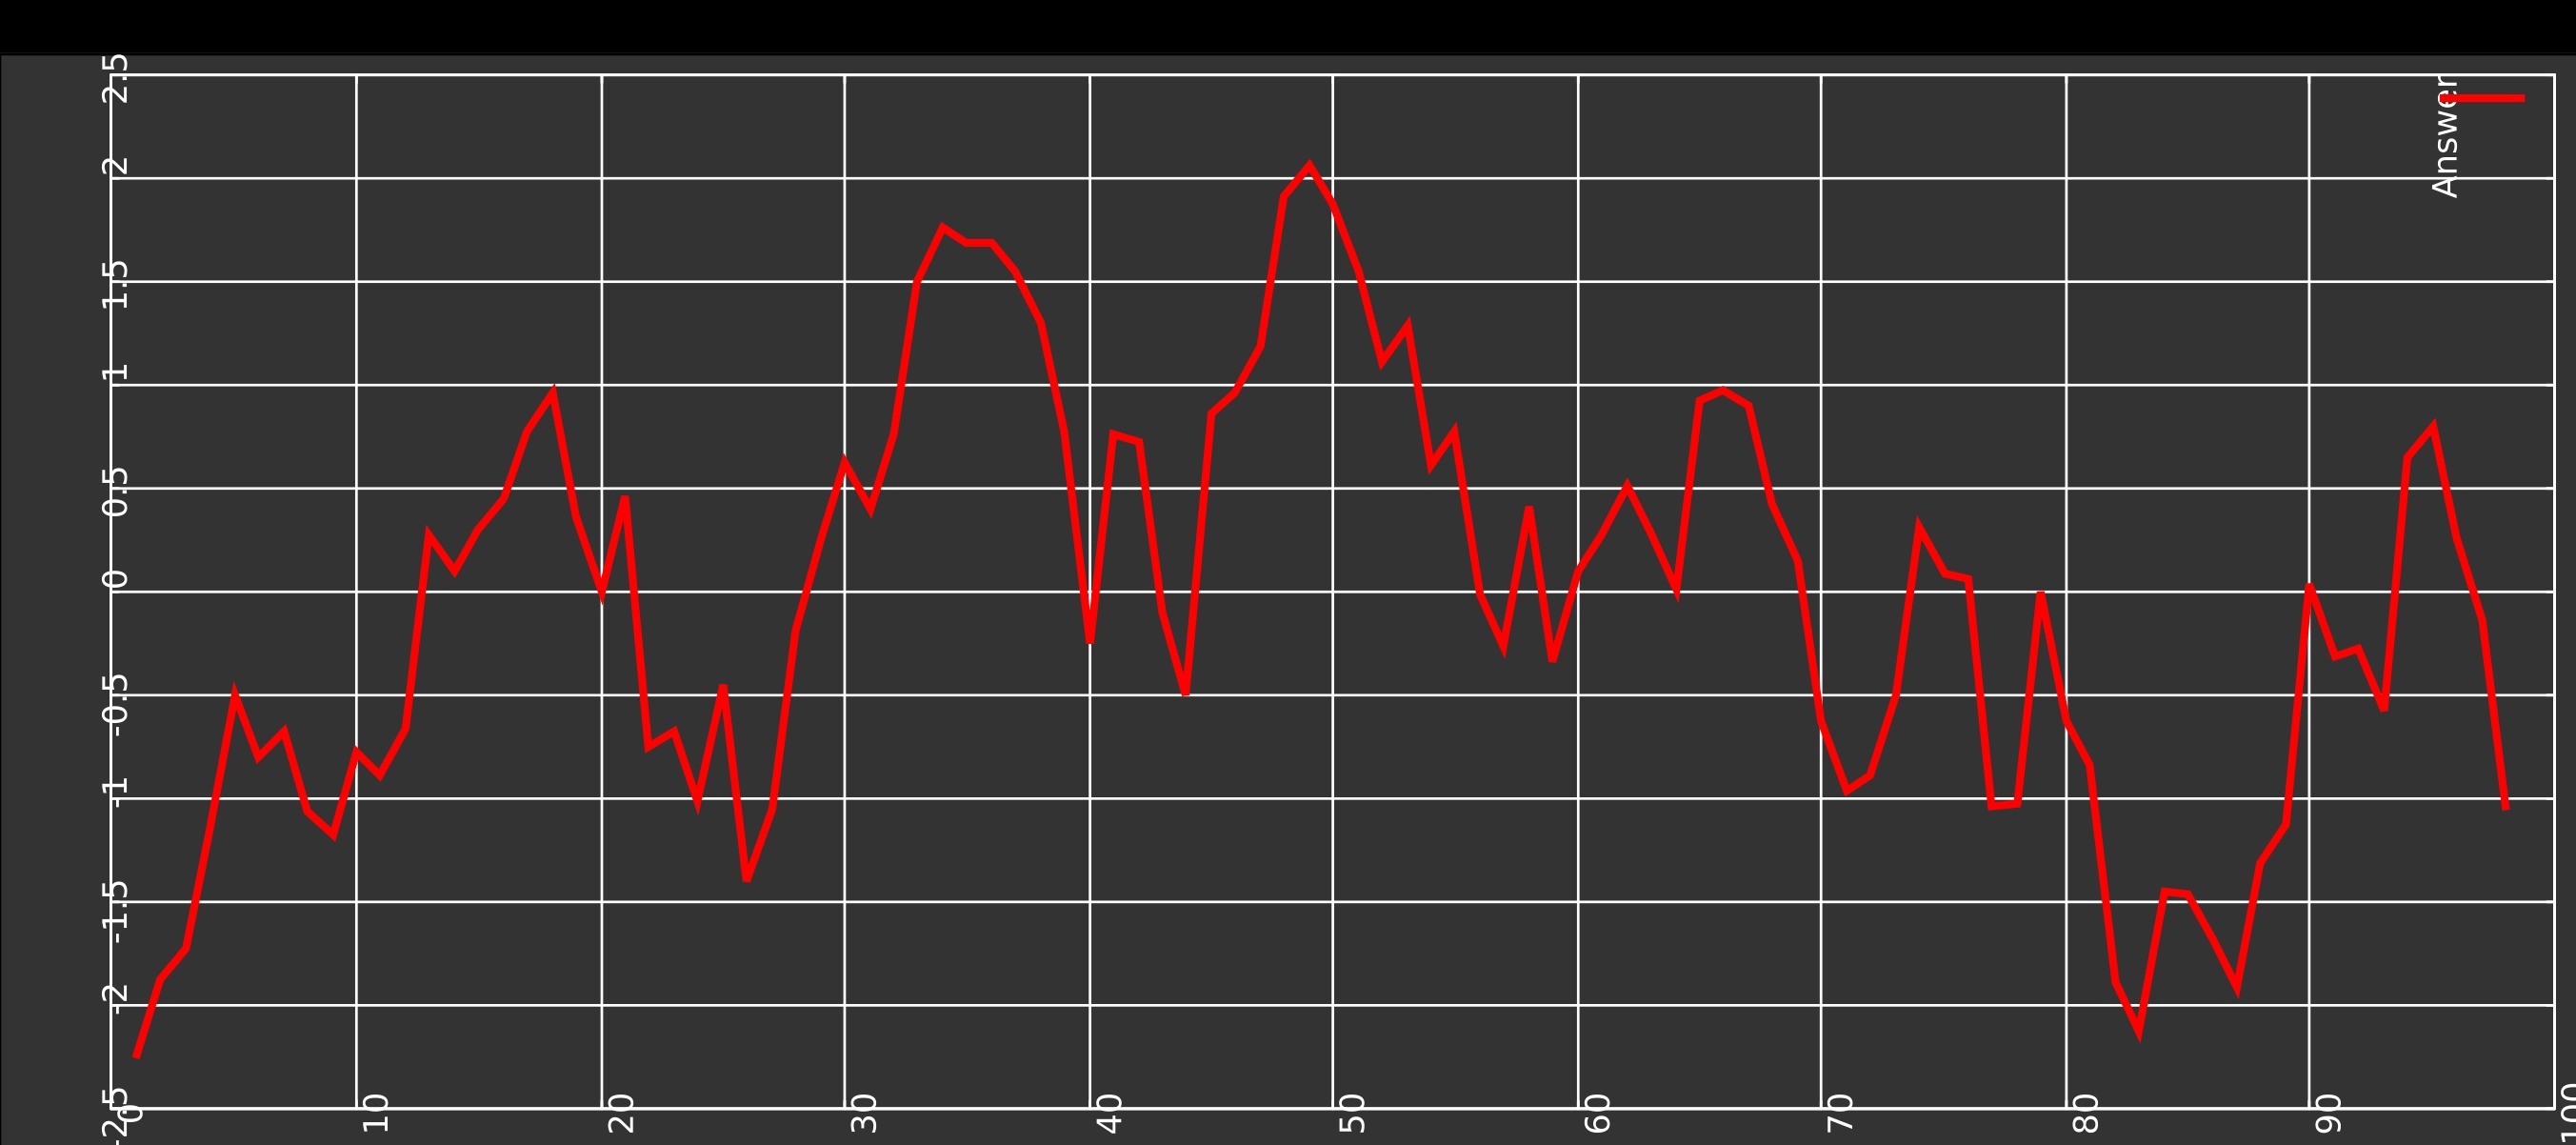
\includegraphics[width=160mm]{X.jpg}
 \end{center}
 \caption{発生したX}
 \label{fig:one}
\end{figure}
上記の式で発生したDRを正規分布関数の逆関数で変換したものが,下記になります。
\begin{figure}[H]
 \begin{center}
  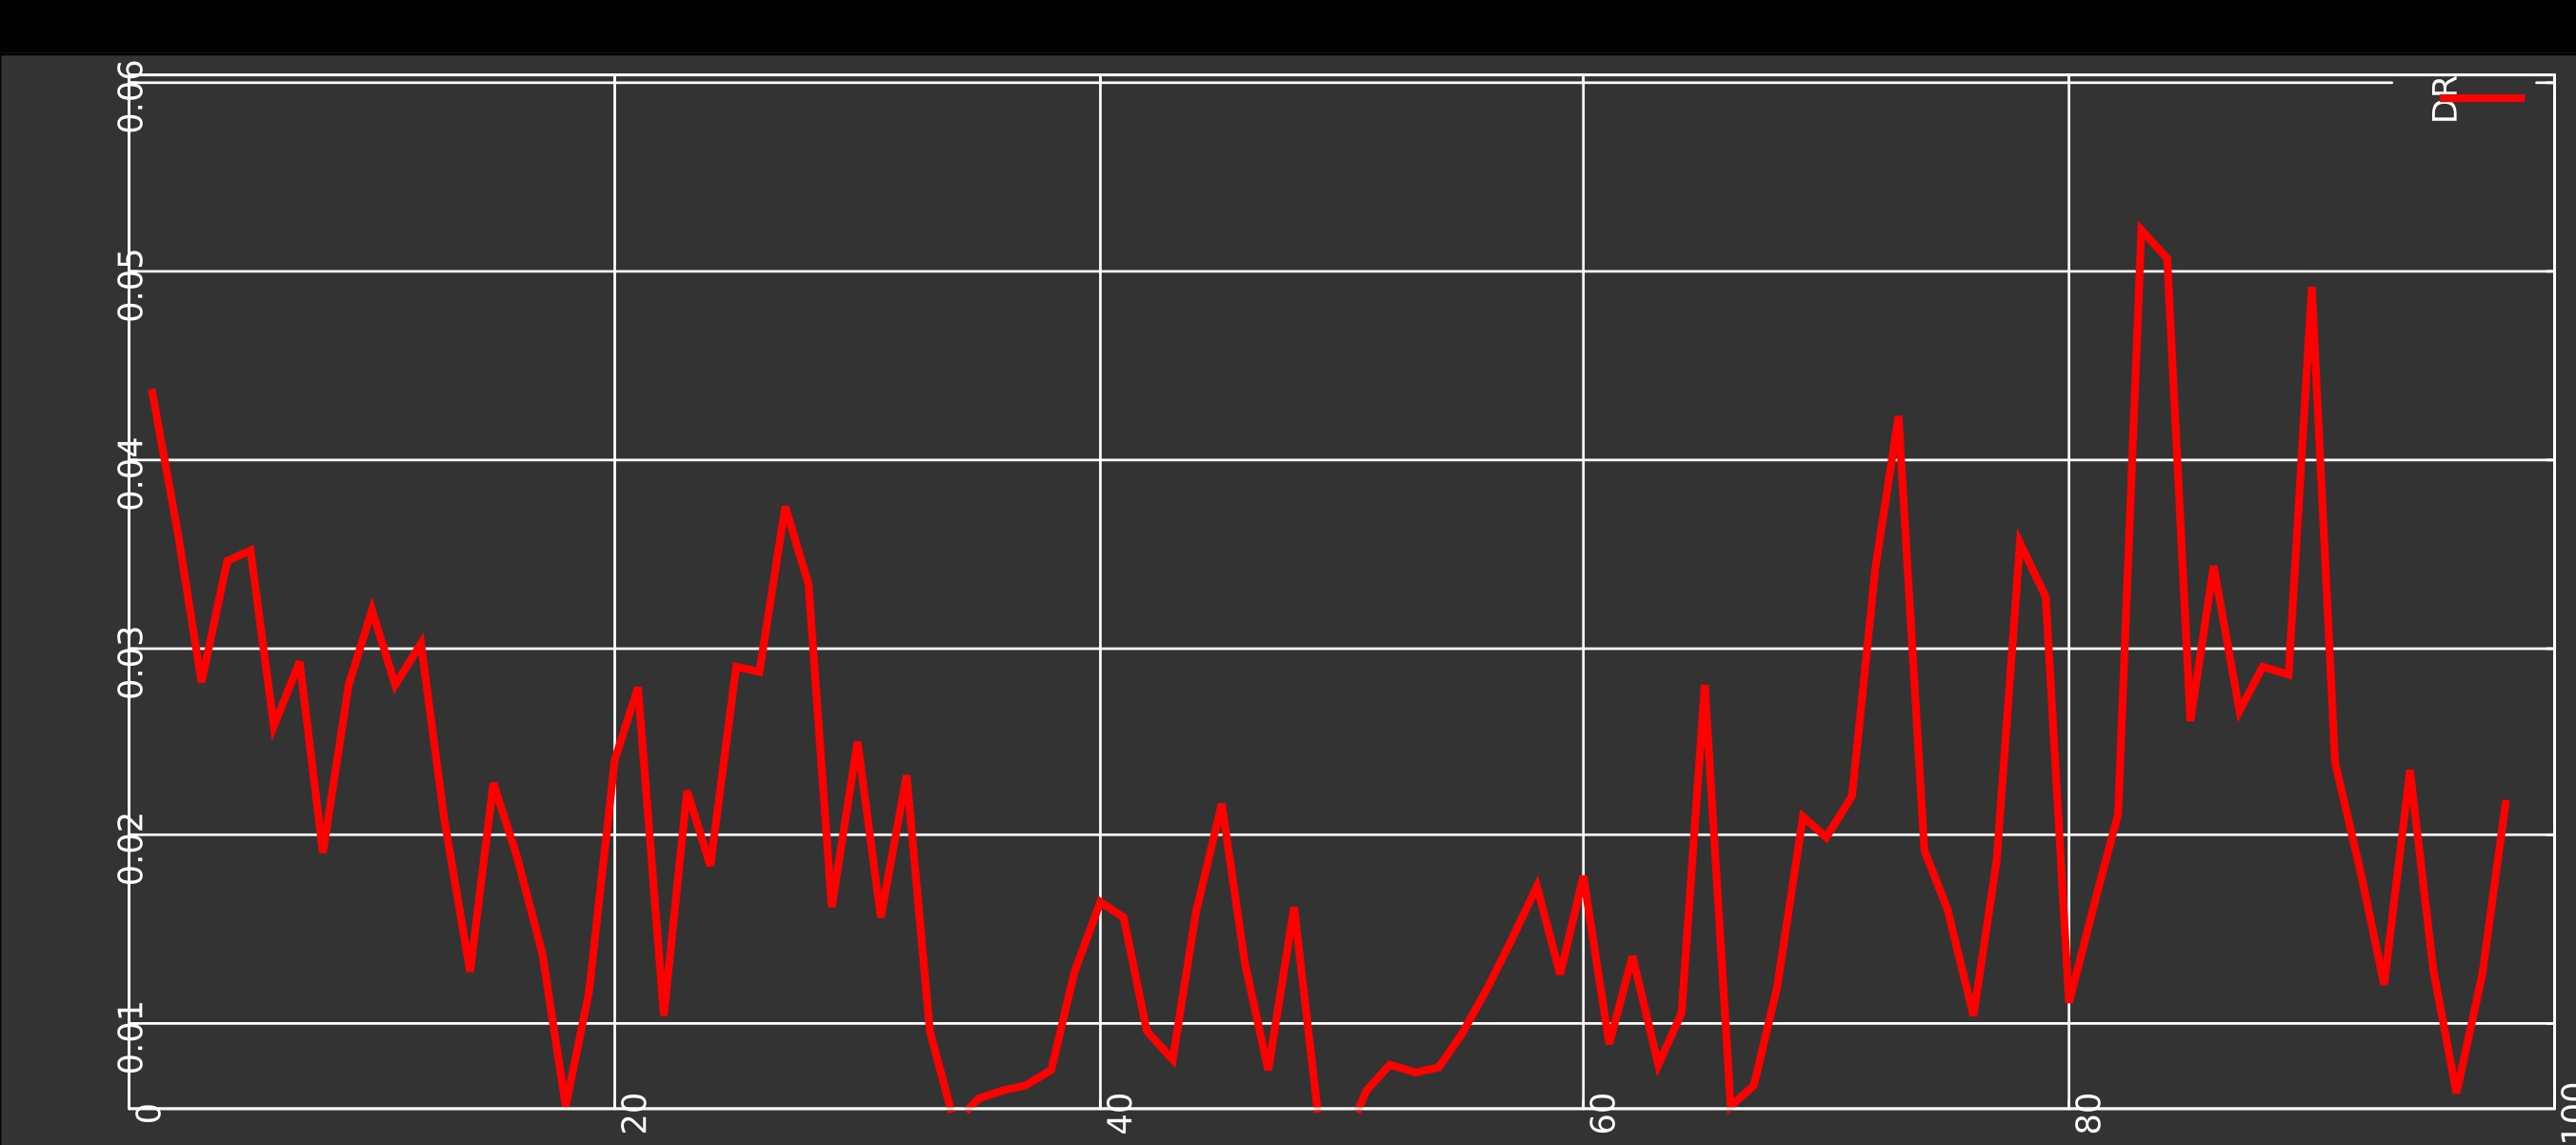
\includegraphics[width=160mm]{DR.jpg}
 \end{center}
 \caption{発生したDR}
 \label{fig:one}
\end{figure}

\section{フィルタリング}
フィルタリングは、Particle数1000個で回しています。提案分布は、実際の分布にしてあります。\\
EMアルゴリズムを行う際には、実際と違うパラメータを用いて行いますが、ここでは正しいパラメータを用いて行います。\\
以下、コードの内容を伝えます。
まず、次の式に従うように、時点0のサンプルを発生させます。
$$
X_0^{(i)}  = \sqrt{\beta}X_0 - \sqrt{1 - \beta}\epsilon_i \hspace{5mm}  \epsilon^{(i)} \sim N(0,1)
$$
各Particleのweightは、下記の尤度より与えています。
$$
\mu_0^{(i)} = \frac{\Phi^{-1}(q)-\sqrt{\rho}\sqrt{\beta}X_0^{(i)}}{\sqrt{1-\rho}} \hspace{5mm}
\sigma = \sqrt{ \frac{\rho(1 - \beta)}{1 - \rho}}
$$
$$
weight_1^{(i)} = \frac{1}{\sqrt{2\pi}\sigma}\exp\left\{-\frac{(DR_1-\mu_0^{(i)})^2}{2\sigma^2}\right\}
$$
$\sum\frac{1}{{weight^{(i)}}^2} < \frac{N}{10}=100$ならばリサンプリングします。

以降は次の繰り返し
$$
X_t^{(i)}  = \sqrt{\beta}X_{t-1}^{(i)} - \sqrt{1 - \beta}\epsilon_i \hspace{5mm}  \epsilon^{(i)} \sim N(0,1)
$$
各Particleのweightは、尤度と前回のweightの積で与えます。
$$
\mu_t^{(i)} = \frac{\Phi^{-1}(q)-\sqrt{\rho}\sqrt{\beta}X_{t-1}^{(i)}}{\sqrt{1-\rho}} \hspace{5mm}
\sigma = \sqrt{ \frac{\rho(1 - \beta)}{1 - \rho}}
$$
$$
weight_t^{(i)} = weight_{t-1}^{(i)} \frac{1}{\sqrt{2\pi}\sigma}\exp\left\{-\frac{(DR_t-\mu_t^{(i)})^2}{2\sigma^2}\right\}
$$
\begin{figure}[H]
 \begin{center}
  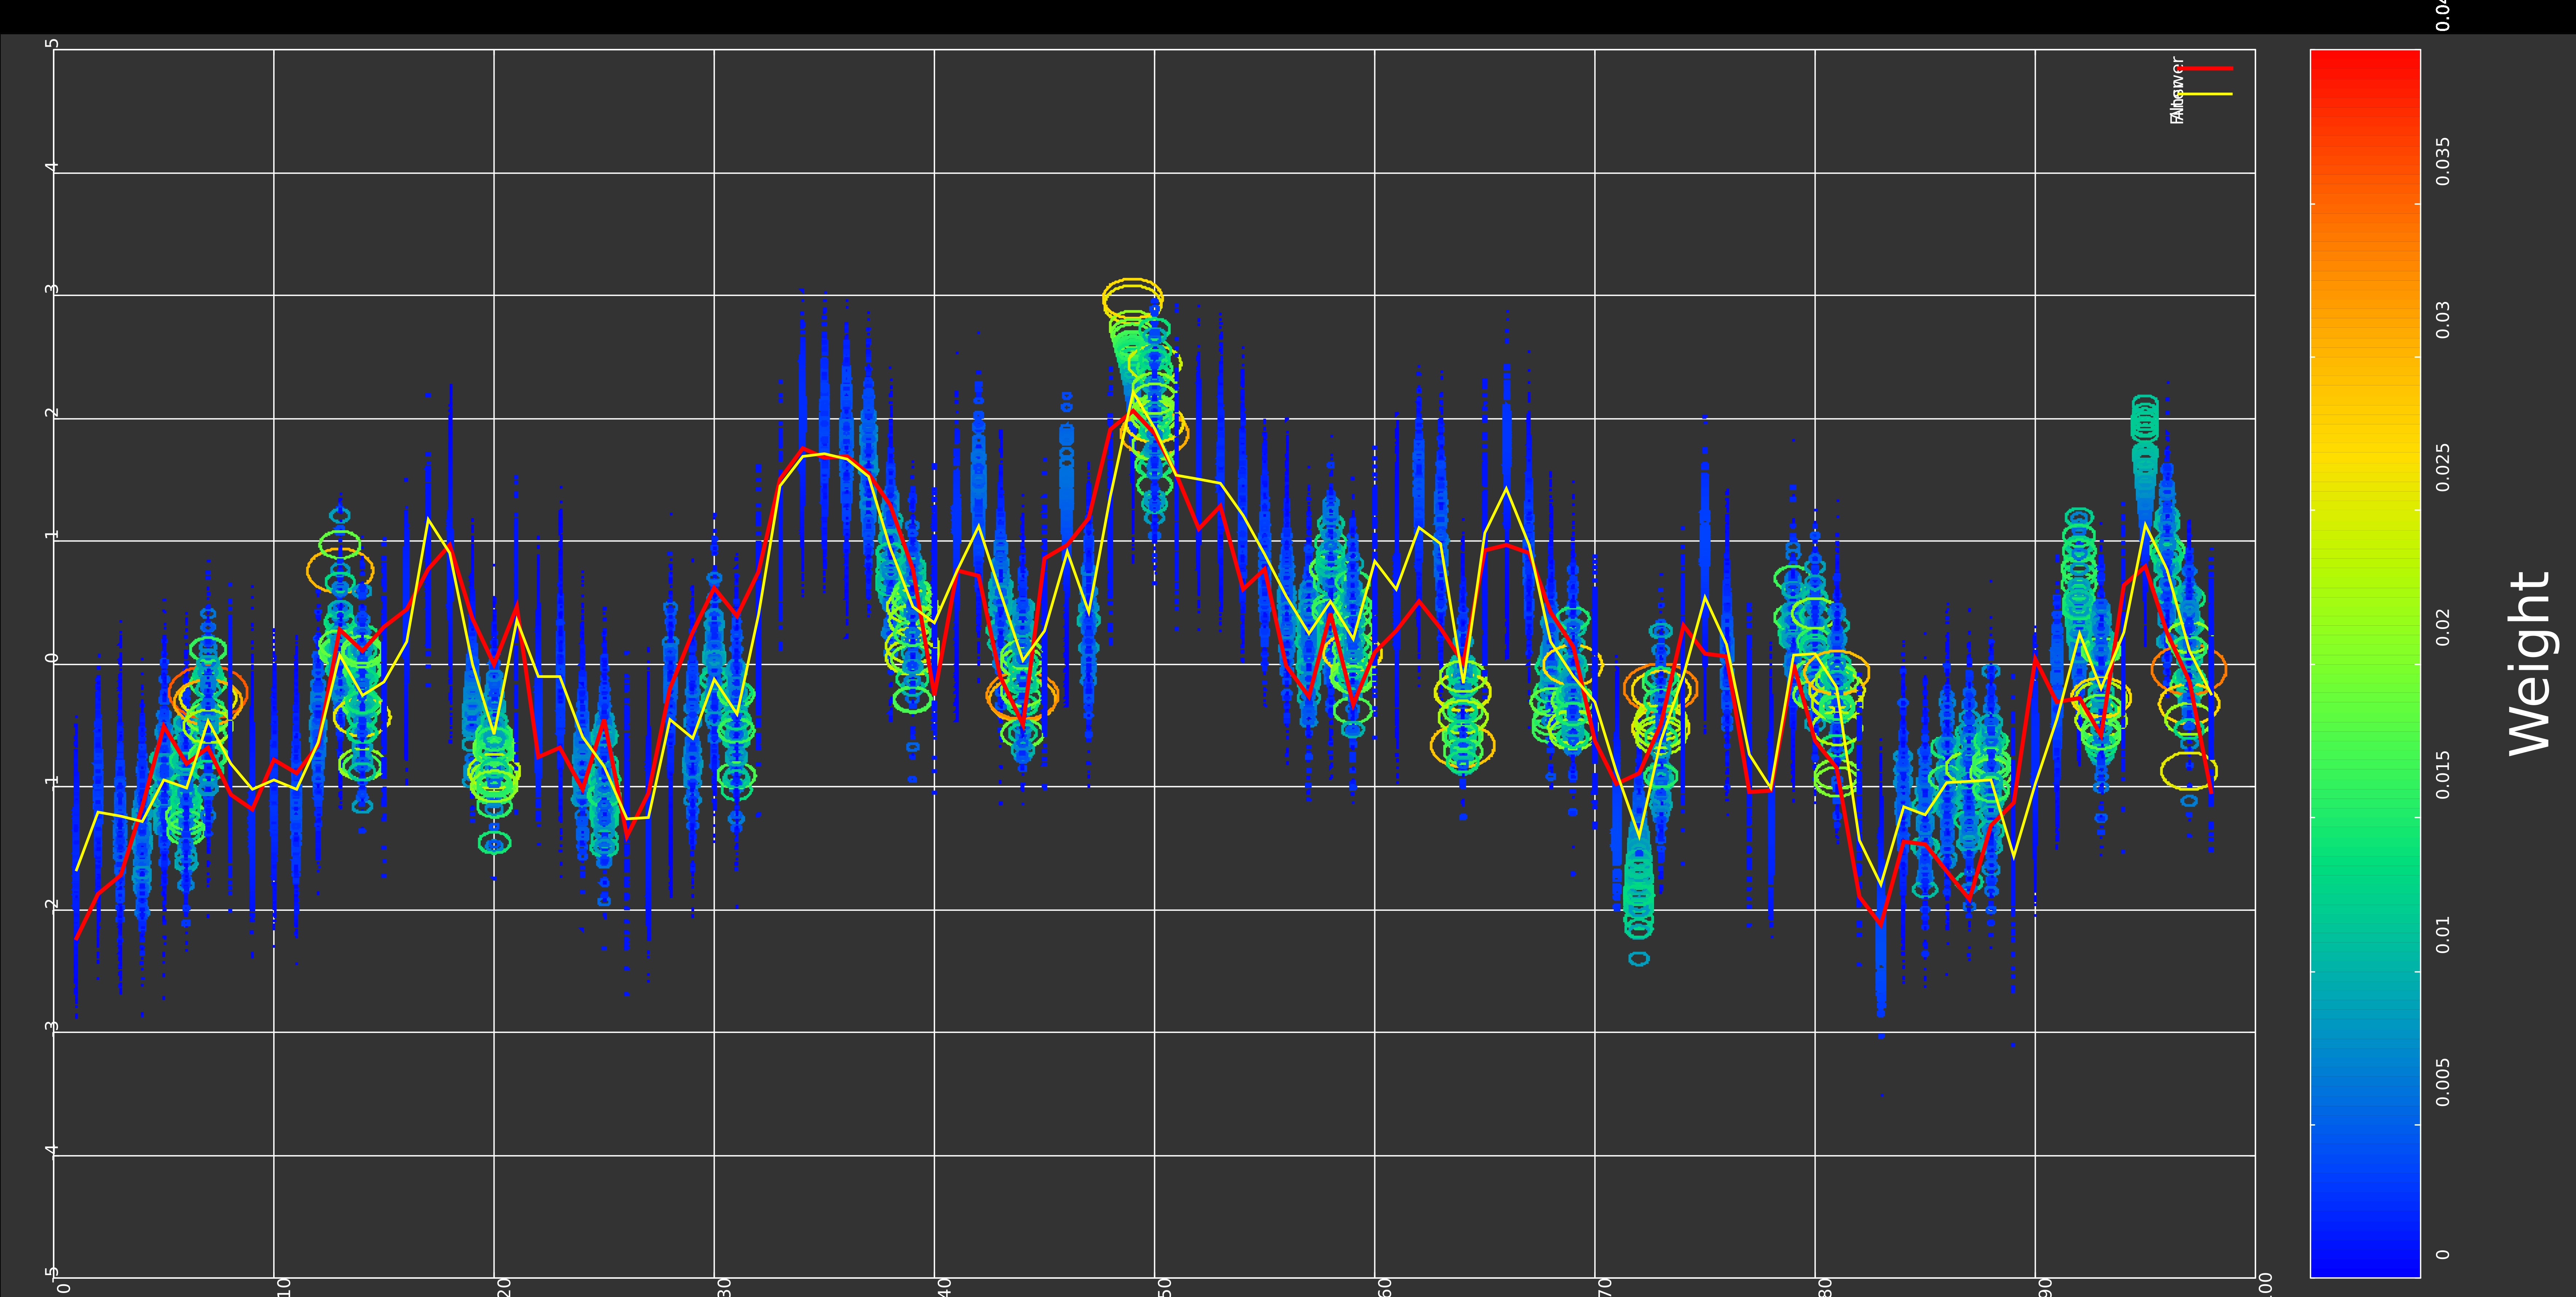
\includegraphics[width=160mm]{Filter.jpg}
 \end{center}
 \caption{Filterlingの結果(赤線が答えで、黄線がフィルタリング)}
 \label{fig:one}
\end{figure}

\section{平滑化}
FFBSによる平滑化です。こちらも、前回のフィルタリングの結果を引きつぎ、正しいパラメータを用いて平滑化を行っています。
計算式は下記の通り、
$$
W_{t|T}^{(i)}=W_t^{(i)}\left(\sum_{j=1}^{N}W_{t+1|T}^{(j)} \frac{f_\theta(X^{(j)}_{t+1}|X^{(i)}_t)}{\sum_{l=1}^N W_t^{l} f_\theta(X^{(i)}_{t+1}|X^{(l)}_t)}\right)
$$
$W_{T|T}^{(i)}$はフィルタリング時の$weight_{T}^{(i)}$で、$W_{t}^{(i)}$はフィルタリング時の$weight_{t}^{(i)}$です。
今回の、$f_\theta(A,B)$は
$$
f_\theta(X_{t+1},X_t)=\frac{1}{\sqrt{2\pi}\sqrt{1 - \beta}}exp\left\{-\frac{(X_{t+1}-\sqrt{\beta}X_{t})^2}{2(1 - \beta)} \right\}
$$
となっています。7月14日22時の時点で、ここまでの処理が約8秒で終了します。
\begin{figure}[H]
 \begin{center}
  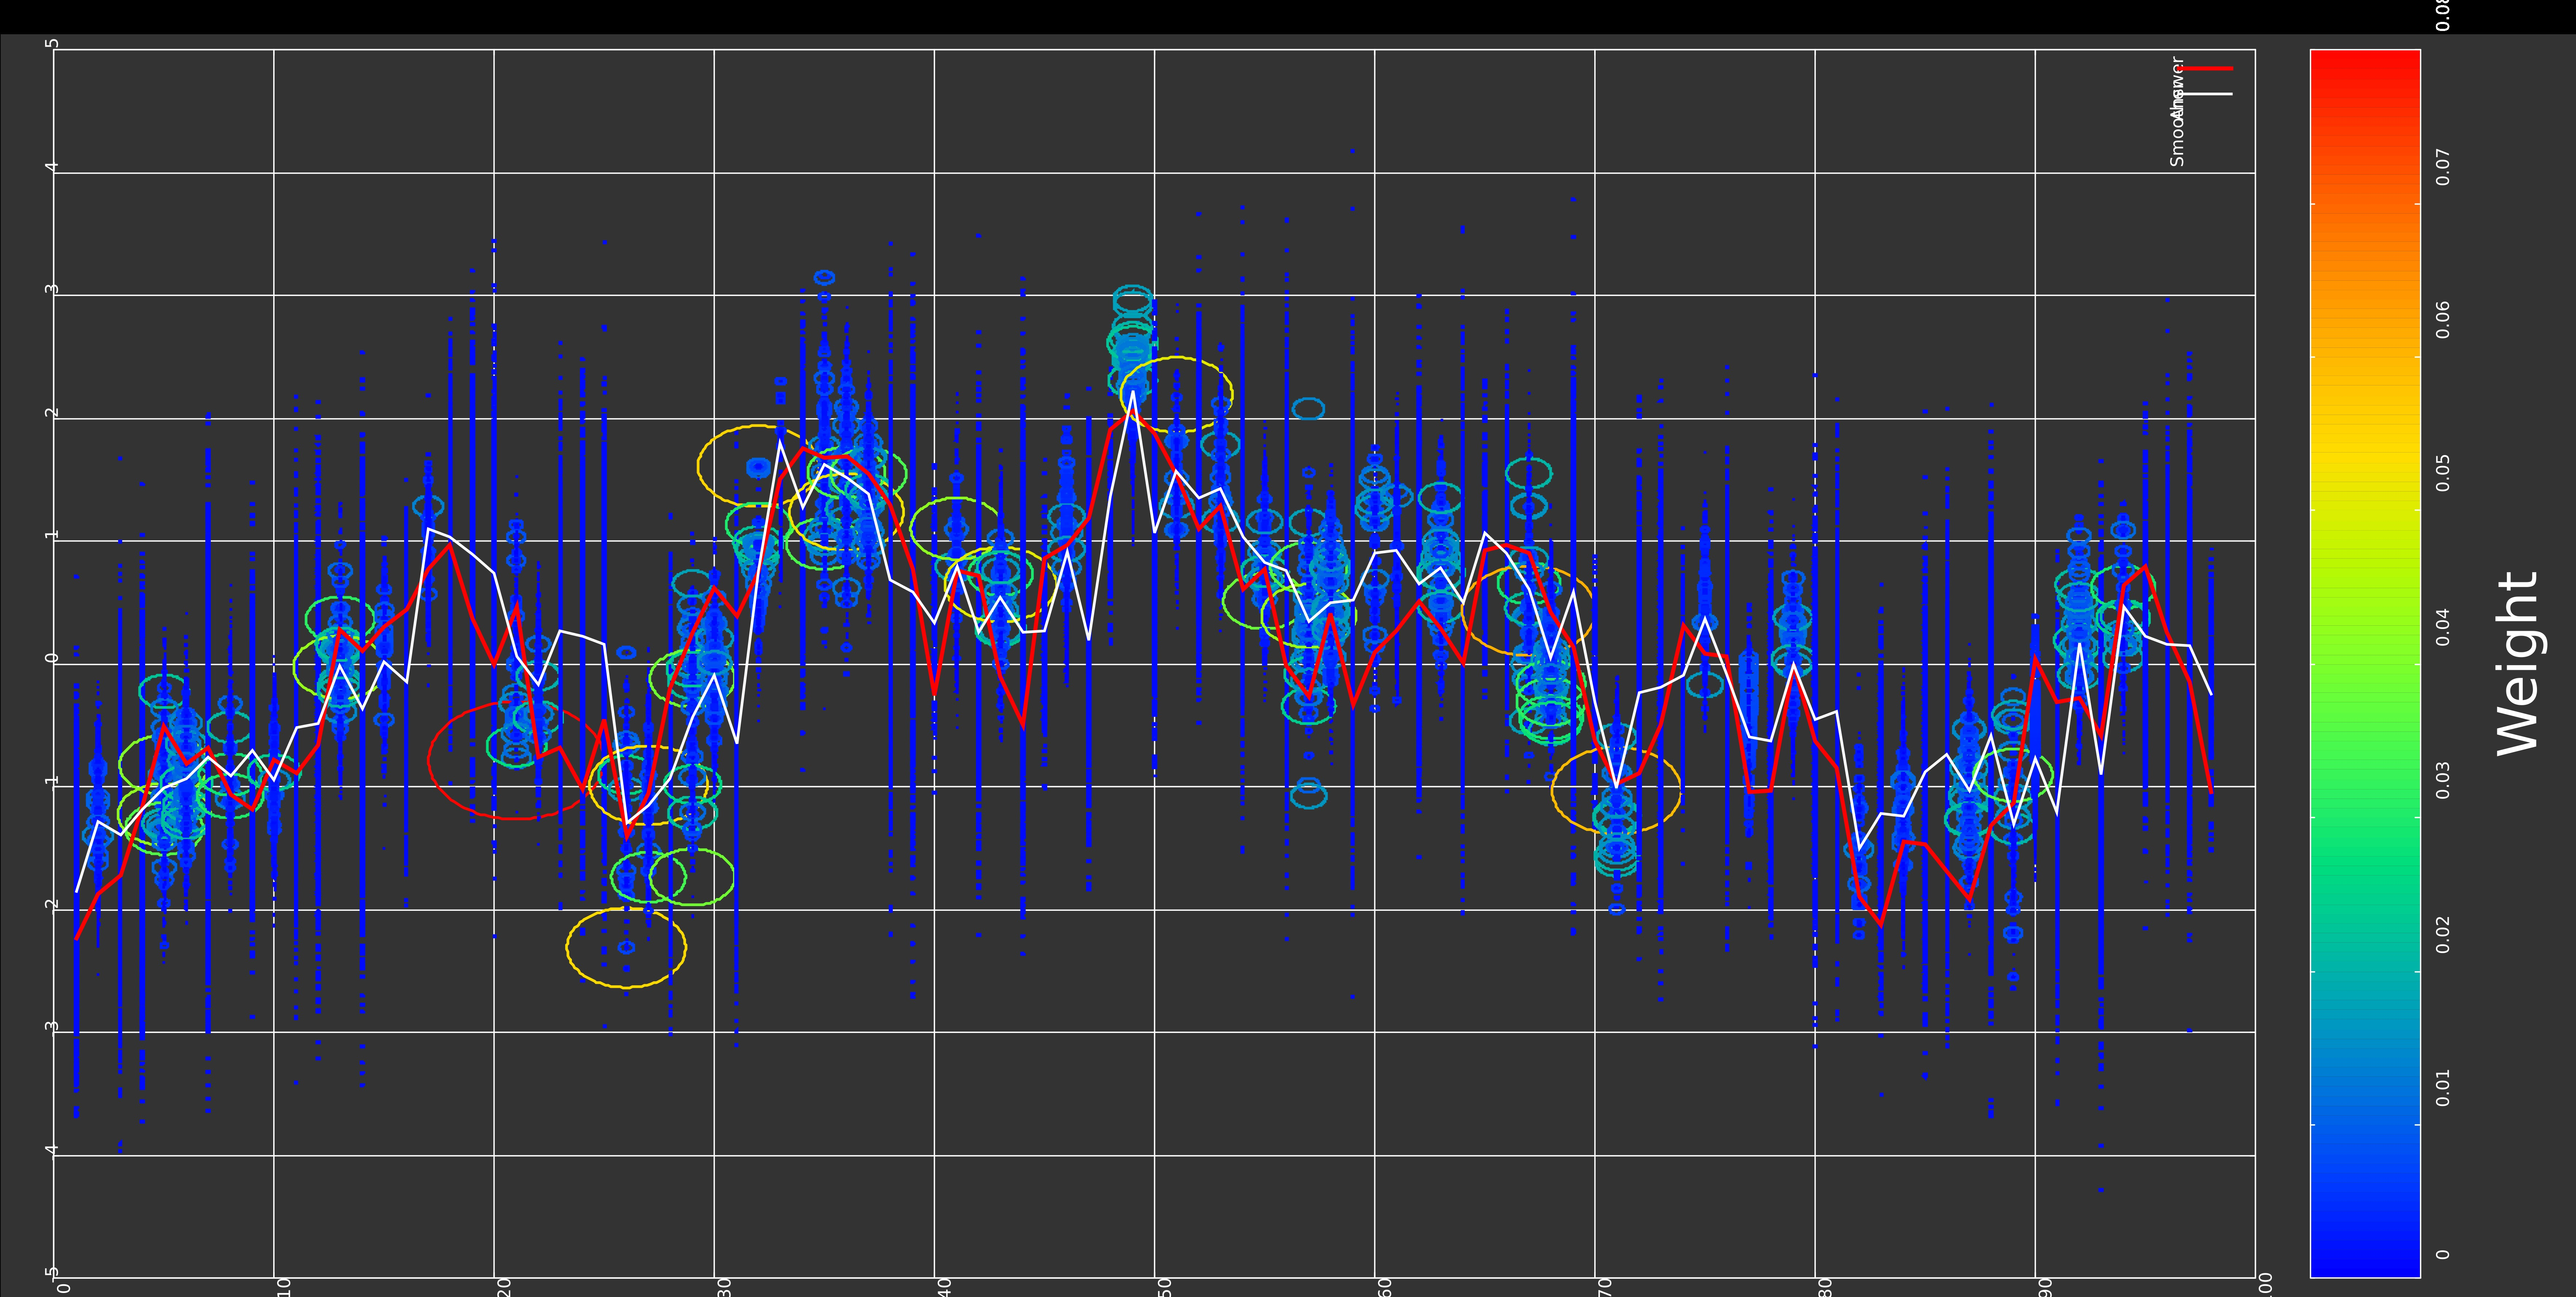
\includegraphics[width=160mm]{Smoother.jpg}
 \end{center}
 \caption{Smoothingの結果(赤線が答えで、白線がSomoothing)}
 \label{fig:one}
\end{figure}
\section{EMアルゴリズム}
FFBSの結果を用いて、パラメータを最適化していきます。
C言語で実装しようとしたところ、最適化計算に用ライブラリが存在しないようなので、自力で組もうとしています。


EMアルゴリズムでは、フィルタリングと平滑化を行った後に、目的関数Qを最大化するようにパラメータを探します。ちなみに、最初に頂いたペーパーとNonlinear Time Seriesの本では、2項目の計算方法が違いました。本にまとめらている方が、FFBSで平滑化を行った場合のEMだったので、こちらを参考にしています。目的関数Qを本のものを引用すると
\begin{eqnarray*}
Q&=&\sum_{i=1}^NW_{0|n}^{(i)}logp^\theta(X_0^{(i)})\hspace{10mm}初期分布から、各初期Particleが発生する対数尤度\\
&+&\sum_{t=1}^{n}\sum_{i=1}^{N}\sum_{j=1}^{N}W_{i|N}^{ij}log f_\theta(X_{t}^{(i)},X_{t-1}^{(j)})\hspace{10mm}各Particleが次のParticleに行く対数尤度\\
&+&\sum_{t=1}^{n}\sum_{i=1}^{N}W_{i|N}^{(i)}logg_\theta(Y_t|X_t^{(i)})\hspace{10mm}各Particleから観測値が得られる対数尤度
\end{eqnarray*}
Dynamic Default Ratesで実装する場合は以下のようになります、パラメータが分かりやすいように色字にしています。添え字も修正しています。
\begin{eqnarray*}
Q&=&\sum_{i=1}^NW_{0|N}^{(i)}log\left(\frac{1}{\sqrt{2\pi}\sqrt{1 - \textcolor{red}{\beta}}}exp\left\{-\frac{(X_{0}^{(i)}-\sqrt{\textcolor{red}{\beta}}\textcolor{green}{X_0})^2}
{2(1 - \textcolor{red}{\beta})} \right\}\right)\\
&+&\sum_{t=1}^{n}\sum_{i=1}^{N}\sum_{j=1}^{N}W_{i|N}^{ij}log \left(\frac{1}{\sqrt{2\pi}\sqrt{1 - \textcolor{red}{\beta}}}exp\left\{-\frac{(X_{t}^{(i)}-\sqrt{\textcolor{red}{\beta}}X_{t-1}^{(j)})^2}
{2(1 - \textcolor{red}{\beta})} \right\}\right)\\
&+&\sum_{t=1}^{n}\sum_{i=1}^{N}W_{i|N}^{(i)}log\left(\frac{1}{\sqrt{2\pi}\sqrt{ \frac{ \textcolor{blue}{\rho}(1 - \textcolor{red}{\beta})}{1 -  \textcolor{blue}{\rho}}}}
\exp\left\{-\frac{(DR_t-(\frac{\Phi^{-1}(\textcolor{magenta}{q})-\sqrt{ \textcolor{blue}{\rho}}\sqrt{\textcolor{red}{\beta}}X_{t-1}^{(i)}}{\sqrt{1- \textcolor{blue}{\rho}}}))^2}{2 \frac{ \textcolor{blue}{\rho}(1 - \textcolor{red}{\beta})}{1 -  \textcolor{blue}{\rho}}}\right\}\right)
\end{eqnarray*}
パラメータ最適化のために、勾配を計算する必要がありますが、次の3つのパラメータは制約や偏微分に問題があり、それぞれ対処します。
\begin{itemize}
 \item $\beta$\hspace{5mm}$\beta$は、定義上(0,1)の範囲しかとらない。 よってシグモイド関数によって変換した$\beta_{sig}$でパラメータ推定を行う。
 \item $\rho$\hspace{5mm}$\rho$も同様。 よってシグモイド関数によって変換したもの$\rho_{sig}$でパラメータ推定を行う。
 \item $q$\hspace{5mm}$q$は、$\Phi^{-1}(q)$が偏微分できない(そもそも$\Phi^{-1}(q)$が近似式によって求まっている)。よって、$\Phi^{-1}(q)$をパラメータとして推定を行う($q_{Inv}$と表す)。
\end{itemize}
それぞれのパラメータを変換させた結果、$Q$の式が以下のように変換されます。
\begin{eqnarray*}
Q&=&\sum_{i=1}^NW_{0|N}^{(i)}log\left(\frac{1}{\sqrt{2\pi}\sqrt{1 - \frac{1}{1+e^{-\textcolor{red}{\beta_{sig}}}}}}exp\left\{-\frac{(X_{0}^{(i)}-\sqrt{\frac{1}{1+e^{-\textcolor{red}{\beta_{sig}}}}}\textcolor{green}{X_0})^2}
{2(1 - \frac{1}{1+e^{-\textcolor{red}{\beta_{sig}}}})} \right\}\right)\\
&+&\sum_{t=1}^{T}\sum_{i=1}^{N}\sum_{j=1}^{N}W_{i|N}^{ij}log \left(\frac{1}{\sqrt{2\pi}\sqrt{1 - \frac{1}{1+e^{-\textcolor{red}{\beta_{sig}}}}}}exp\left\{-\frac{(X_{t}^{(i)}-\sqrt{\frac{1}{1+e^{-\textcolor{red}{\beta_{sig}}}}}X_{t-1}^{(j)})^2}
{2(1 - \frac{1}{1+e^{-\textcolor{red}{\beta_{sig}}}})} \right\}\right)\\
&+&\sum_{t=1}^{T}\sum_{i=1}^{N}W_{i|N}^{(i)}log\left(\frac{1}{\sqrt{2\pi}\sqrt{ \frac{\frac{1}{1+e^{-\textcolor{blue}{\rho_{sig}}}} (1 - \frac{1}{1+e^{-\textcolor{red}{\beta_{sig}}}})}{1 -  \frac{1}{1+e^{-\textcolor{blue}{\rho_{sig}}}}}}}
\exp\left\{-\frac{\left(DR_t-\left(\frac{\textcolor{magenta}{q_{Inv}}-\sqrt{ \frac{1}{1+e^{-\textcolor{blue}{\rho_{sig}}}}}\sqrt{\frac{1}{1+e^{-\textcolor{red}{\beta_{sig}}}}}X_{t-1}^{(i)}}{\sqrt{1- \frac{1}{1+e^{-\textcolor{blue}{\rho_{sig}}}}}}\right)\right)^2}{2 \frac{ \frac{1}{1+e^{-\textcolor{blue}{\rho_{sig}}}}(1 - \frac{1}{1+e^{-\textcolor{red}{\beta_{sig}}}})}{1 -  \frac{1}{1+e^{-\textcolor{blue}{\rho_{sig}}}}}}\right\}\right)
\end{eqnarray*}
各項について、整理しておきます。
\begin{eqnarray*}
第1項&=&\sum_{i=1}^NW_{0|N}^{(i)}log\left(\frac{1}{\sqrt{2\pi}\sqrt{1 - \frac{1}{1+e^{-\textcolor{red}{\beta_{sig}}}}}}exp\left\{-\frac{(X_{0}^{(i)}-\sqrt{\frac{1}{1+e^{-\textcolor{red}{\beta_{sig}}}}}\textcolor{green}{X_0})^2}
{2(1 - \frac{1}{1+e^{-\textcolor{red}{\beta_{sig}}}})} \right\}\right)\\
&=&\sum_{i=1}^NW_{0|N}^{(i)} \left(-\frac{1}{2} log\left[2\pi  \frac{ {e^{-\textcolor{red}{\beta_{sig}}}}}{1 + e^{-\textcolor{red}{\beta_{sig}}}}\right]-\left(\frac{(X_{0}^{(i)}-\sqrt{\frac{1}{1+e^{-\textcolor{red}{\beta_{sig}}}}}\textcolor{green}{X_0})^2}
{2(\frac{e^{-\textcolor{red}{\beta_{sig}}}}{1+e^{-\textcolor{red}{\beta_{sig}}}})} \right)\right)\\
&=&\sum_{i=1}^NW_{0|N}^{(i)}\left(-\frac{e^{\textcolor{red}{\beta_{sig}}}}{2}(1+e^{-\textcolor{red}{\beta_{sig}}})\left( {X_0^{(i)}}^2 -2\sqrt{\frac{1}{1+e^{-\textcolor{red}{\beta_{sig}}}}}X_0^{(i)}\textcolor{green}{X_0} + \frac{1}{1+e^{-\textcolor{red}{\beta_{sig}}}}\textcolor{green}{X_0}^2 \right) - \frac{1}{2}(log\left[2\pi\right] - log\left[1 + e^{\textcolor{red}{\beta_{sig}}}\right])\right)\\
&=&\sum_{i=1}^NW_{0|N}^{(i)} \left(-\frac{e^{\textcolor{red}{\beta_{sig}}}}{2}\left((1+e^{-\textcolor{red}{\beta_{sig}}}){X_0^{(i)}}^2 -2\sqrt{(1+e^{-\textcolor{red}{\beta_{sig}}})}X_0^{(i)}\textcolor{green}{X_0} + \textcolor{green}{X_0}^2 \right)-\frac{1}{2}(log\left[2\pi\right] - log\left[1 + e^{\textcolor{red}{\beta_{sig}}}\right])\right)\\
第2項&=&\sum_{t=1}^{T}\sum_{i=1}^{N}\sum_{j=1}^{N}W_{i|N}^{ij}log \left(\frac{1}{\sqrt{2\pi}\sqrt{1 - \frac{1}{1+e^{-\textcolor{red}{\beta_{sig}}}}}}exp\left\{-\frac{(X_{t}^{(i)}-\sqrt{\frac{1}{1+e^{-\textcolor{red}{\beta_{sig}}}}}X_{t-1}^{(j)})^2}
{2(1 - \frac{1}{1+e^{-\textcolor{red}{\beta_{sig}}}})} \right\}\right)(第1項と同様に変形)\\
&=&\sum_{t=1}^{T}\sum_{i=1}^{N}\sum_{j=1}^{N}W_{i|N}^{ij} \left(-\frac{e^{\textcolor{red}{\beta_{sig}}}}{2}\left((1+e^{-\textcolor{red}{\beta_{sig}}}){X_t^{(i)}}^2 -2\sqrt{(1+e^{-\textcolor{red}{\beta_{sig}}})}X_t^{(i)}X_{t-1}^{(j)} + {X_{t-1}^{(j)}}^2 \right)-\frac{1}{2}(log\left[2\pi\right] - log\left[1 + e^{\textcolor{red}{\beta_{sig}}}\right])\right)\\
\end{eqnarray*}
\begin{eqnarray*}
第3項&=&\sum_{t=1}^{T}\sum_{i=1}^{N}W_{i|N}^{(i)}log\left(\frac{1}{\sqrt{2\pi}\sqrt{ \frac{\frac{1}{1+e^{-\textcolor{blue}{\rho_{sig}}}} (1 - \frac{1}{1+e^{-\textcolor{red}{\beta_{sig}}}})}{1 -  \frac{1}{1+e^{-\textcolor{blue}{\rho_{sig}}}}}}}
\exp\left\{-\frac{\left(DR_t-\left(\frac{\textcolor{magenta}{q_{Inv}}-\sqrt{ \frac{1}{1+e^{-\textcolor{blue}{\rho_{sig}}}}}\sqrt{\frac{1}{1+e^{-\textcolor{red}{\beta_{sig}}}}}X_{t-1}^{(i)}}{\sqrt{1- \frac{1}{1+e^{-\textcolor{blue}{\rho_{sig}}}}}}\right)\right)^2}{2 \frac{ \frac{1}{1+e^{-\textcolor{blue}{\rho_{sig}}}}(1 - \frac{1}{1+e^{-\textcolor{red}{\beta_{sig}}}})}{1 -  \frac{1}{1+e^{-\textcolor{blue}{\rho_{sig}}}}}}\right\}\right)\\
&=&\sum_{t=1}^{T}\sum_{i=1}^{N}W_{i|N}^{(i)}\left(-\frac{1}{2} log\left[2\pi \frac{e^{\textcolor{blue}{\rho_{sig}}}}{1+e^{\textcolor{red}{\beta_{sig}}}}\right]
-\left\{\frac{\left(DR_t-\left(\frac{\textcolor{magenta}{q_{Inv}}-\sqrt{ \frac{1}{1+e^{-\textcolor{blue}{\rho_{sig}}}}}\sqrt{\frac{1}{1+e^{-\textcolor{red}{\beta_{sig}}}}}X_{t-1}^{(i)}}{\sqrt{\frac{e^{-\textcolor{blue}{\rho_{sig}}}}{1+e^{-\textcolor{blue}{\rho_{sig}}}}}}\right)\right)^2}{2 \frac{e^{\textcolor{blue}{\rho_{sig}}}}{1+e^{\textcolor{red}{\beta_{sig}}}}}\right\}\right)\\
&=&\sum_{t=1}^{T}\sum_{i=1}^{N}W_{i|N}^{(i)}\left( -\frac{1}{2} log\left[2\pi \frac{e^{\textcolor{blue}{\rho_{sig}}}}{1+e^{\textcolor{red}{\beta_{sig}}}}\right]
-\frac{(1+e^{\textcolor{red}{\beta_{sig}}})}{2e^{\textcolor{blue}{\rho_{sig}}}}\left\{\left(DR_t-\left(\frac{\textcolor{magenta}{q_{Inv}}-\sqrt{ \frac{1}{1+e^{-\textcolor{blue}{\rho_{sig}}}}}\sqrt{\frac{1}{1+e^{-\textcolor{red}{\beta_{sig}}}}}X_{t-1}^{(i)}}{\sqrt{\frac{e^{-\textcolor{blue}{\rho_{sig}}}}{1+e^{-\textcolor{blue}{\rho_{sig}}}}}}\right)\right)^2\right\} \right)\\
&=&\sum_{t=1}^{T}\sum_{i=1}^{N}W_{i|N}^{(i)}(-\frac{1}{2} log\left[2\pi \frac{e^{\textcolor{blue}{\rho_{sig}}}}{1+e^{\textcolor{red}{\beta_{sig}}}}\right]
-\frac{(1+e^{\textcolor{red}{\beta_{sig}}})}{2e^{\textcolor{blue}{\rho_{sig}}}}\\
&&\left\{DR_t^2-\left(\frac{\textcolor{magenta}{q_{Inv}}-\sqrt{ \frac{1}{1+e^{-\textcolor{blue}{\rho_{sig}}}}}\sqrt{\frac{1}{1+e^{-\textcolor{red}{\beta_{sig}}}}}X_{t-1}^{(i)}}{\sqrt{\frac{e^{-\textcolor{blue}{\rho_{sig}}}}{1+e^{-\textcolor{blue}{\rho_{sig}}}}}}\right)^2 - 2DR_t
\left(\frac{\textcolor{magenta}{q_{Inv}}-\sqrt{ \frac{1}{1+e^{-\textcolor{blue}{\rho_{sig}}}}}\sqrt{\frac{1}{1+e^{-\textcolor{red}{\beta_{sig}}}}}X_{t-1}^{(i)}}{\sqrt{\frac{e^{-\textcolor{blue}{\rho_{sig}}}}{1+e^{-\textcolor{blue}{\rho_{sig}}}}}}\right)
 \right\}\\
&&)\\
&=&\sum_{t=1}^{T}\sum_{i=1}^{N}W_{i|N}^{(i)}(-\frac{1}{2} log\left[2\pi \frac{e^{\textcolor{blue}{\rho_{sig}}}}{1+e^{\textcolor{red}{\beta_{sig}}}}\right]
-\frac{(1+e^{\textcolor{red}{\beta_{sig}}})}{2e^{\textcolor{blue}{\rho_{sig}}}}\\
&&\left\{DR_t^2-\left(\frac{\sqrt{ 1+e^{-\textcolor{blue}{\rho_{sig}}}} \textcolor{magenta}{q_{Inv}}-\sqrt{\frac{1}{1+e^{-\textcolor{red}{\beta_{sig}}}}}X_{t-1}^{(i)}}{\sqrt{e^{-\textcolor{blue}{\rho_{sig}}}}}\right)^2 - 2DR_t
\left(\frac{\sqrt{1+e^{-\textcolor{blue}{\rho_{sig}}}} \textcolor{magenta}{q_{Inv}}-\sqrt{\frac{1}{1+e^{-\textcolor{red}{\beta_{sig}}}}}X_{t-1}^{(i)}}{\sqrt{e^{-\textcolor{blue}{\rho_{sig}}}}}\right)
 \right\}\\
&&)\\
&=&\sum_{t=1}^{T}\sum_{i=1}^{N}W_{i|N}^{(i)}(-\frac{1}{2} log\left[2\pi \frac{e^{\textcolor{blue}{\rho_{sig}}}}{1+e^{\textcolor{red}{\beta_{sig}}}}\right]
-\frac{(1+e^{\textcolor{red}{\beta_{sig}}})}{2e^{\textcolor{blue}{\rho_{sig}}}}\\
&&
\scalebox{0.9}{$\displaystyle
\left\{DR_t^2-
\left((1+ e^{\textcolor{blue}{\rho_{sig}}} ) \textcolor{magenta}{q_{Inv}}^2+\frac{e^{\textcolor{blue}{\rho_{sig}}}}{1+e^{-\textcolor{red}{\beta_{sig}}}}{X_{t-1}^{(i)}}^2 - 2 \sqrt{\frac{e^{\textcolor{blue}{\rho_{sig}}} + e^{2\textcolor{blue}{\rho_{sig}}} }{1+e^{-\textcolor{red}{\beta_{sig}}}} }\textcolor{magenta}{q_{Inv}}X_{t-1}^{(i)}\right)
 - 2DR_t
\left(\sqrt{1+e^{\textcolor{blue}{\rho_{sig}}}} \textcolor{magenta}{q_{Inv}}-\sqrt{\frac{e^{\textcolor{blue}{\rho_{sig}}}}{1+e^{\textcolor{red}{\beta_{sig}}}}}X_{t-1}^{(i)}\right)
 \right\}
$}
\\
&&)\\
&=&\sum_{t=1}^{T}\sum_{i=1}^{N}W_{i|N}^{(i)}
(-\frac{1}{2} \left(log[2\pi] + \textcolor{blue}{\rho_{sig}} - log[1+e^{\textcolor{red}{\beta_{sig}}}]\right)
-\frac{(1+e^{\textcolor{red}{\beta_{sig}}})}{2e^{\textcolor{blue}{\rho_{sig}}}}\\
&&
\scalebox{0.9}{$\displaystyle
\left\{DR_t^2-
\left((1+ e^{\textcolor{blue}{\rho_{sig}}} ) \textcolor{magenta}{q_{Inv}}^2+\frac{e^{\textcolor{blue}{\rho_{sig}}}}{1+e^{-\textcolor{red}{\beta_{sig}}}}{X_{t-1}^{(i)}}^2 - 2 \sqrt{\frac{e^{\textcolor{blue}{\rho_{sig}}} + e^{2\textcolor{blue}{\rho_{sig}}} }{1+e^{-\textcolor{red}{\beta_{sig}}}} }\textcolor{magenta}{q_{Inv}}X_{t-1}^{(i)}\right)
 - 2DR_t
\left(\sqrt{1+e^{\textcolor{blue}{\rho_{sig}}}} \textcolor{magenta}{q_{Inv}}-\sqrt{\frac{e^{\textcolor{blue}{\rho_{sig}}}}{1+e^{-\textcolor{red}{\beta_{sig}}}}}X_{t-1}^{(i)}\right)
 \right\}
$}
\\
&&)
\end{eqnarray*}
上記の式での、各パラメータについて偏微分を行うので、パラメータごとにまとめていきます。
\subsection{$\beta_{sig}$の偏微分}
まず第1項
$$
\sum_{i=1}^NW_{0|N}^{(i)} \left(-\frac{e^{\textcolor{red}{\beta_{sig}}}}{2}\left((1+e^{-\textcolor{red}{\beta_{sig}}}){X_0^{(i)}}^2 -2\sqrt{(1+e^{-\textcolor{red}{\beta_{sig}}})}X_0^{(i)}\textcolor{green}{X_0} + \textcolor{green}{X_0}^2 \right)-\frac{1}{2}(log\left[2\pi\right] - log\left[1 + e^{\textcolor{red}{\beta_{sig}}}\right])\right)
$$
に対する偏微分を行う
\begin{eqnarray}
&&\sum_{i=1}^NW_{0|N}^{(i)}(\nonumber\\
&-&\frac{e^{\textcolor{red}{\beta_{sig}}}}{2}\left((1+e^{-\textcolor{red}{\beta_{sig}}}){X_0^{(i)}}^2 -2\sqrt{(1+e^{-\textcolor{red}{\beta_{sig}}})}X_0^{(i)}\textcolor{green}{X_0} + \textcolor{green}{X_0}^2 \right)\nonumber\\
&-&\frac{e^{\textcolor{red}{\beta_{sig}}}}{2}\left((-e^{-\textcolor{red}{\beta_{sig}}}){X_0^{(i)}}^2 +\frac{e^{-\textcolor{red}{\beta_{sig}}}}{\sqrt{1+e^{-\textcolor{red}{\beta_{sig}}}}}X_0^{(i)}\textcolor{green}{X_0} \right)\nonumber\\
&+&\frac{1}{2}\frac{e^{\textcolor{red}{\beta_{sig}}}}{1+e^{\textcolor{red}{\beta_{sig}}}}\nonumber\\
&&)
\end{eqnarray}
同様にして、第2項が
\begin{eqnarray}
&&\sum_{t=1}^{T}\sum_{i=1}^{N}\sum_{j=1}^{N}W_{i|N}^{ij}(\nonumber\\
&-&\frac{e^{\textcolor{red}{\beta_{sig}}}}{2}\left((1+e^{-\textcolor{red}{\beta_{sig}}}){X_t^{(i)}}^2 -2\sqrt{(1+e^{-\textcolor{red}{\beta_{sig}}})}X_t^{(i)}{X_{t-1}^{(j)}} + {X_{t-1}^{(j)}}^2 \right)\nonumber\\
&-&\frac{e^{\textcolor{red}{\beta_{sig}}}}{2}\left((-e^{-\textcolor{red}{\beta_{sig}}}){X_t^{(i)}}^2 +\frac{e^{-\textcolor{red}{\beta_{sig}}}}{\sqrt{1+e^{-\textcolor{red}{\beta_{sig}}}}}X_t^{(i)}{X_{t-1}^{(j)}} \right)\nonumber\\
&+&\frac{1}{2}\frac{e^{\textcolor{red}{\beta_{sig}}}}{1+e^{\textcolor{red}{\beta_{sig}}}}\nonumber\\
&&)
\end{eqnarray}
また、第3項
\begin{eqnarray*}
&&\sum_{t=1}^{T}\sum_{i=1}^{N}W_{i|N}^{(i)}
(-\frac{1}{2} \left(log[2\pi] + \textcolor{blue}{\rho_{sig}} - log[1+e^{\textcolor{red}{\beta_{sig}}}]\right)
-\frac{(1+e^{\textcolor{red}{\beta_{sig}}})}{2e^{\textcolor{blue}{\rho_{sig}}}}\\
&&
\scalebox{0.95}{$\displaystyle
\left\{DR_t^2-
\left((1+ e^{\textcolor{blue}{\rho_{sig}}} ) \textcolor{magenta}{q_{Inv}}^2+\frac{e^{\textcolor{blue}{\rho_{sig}}}}{1+e^{-\textcolor{red}{\beta_{sig}}}}{X_{t-1}^{(i)}}^2 - 2 \sqrt{\frac{e^{\textcolor{blue}{\rho_{sig}}} + e^{2\textcolor{blue}{\rho_{sig}}} }{1+e^{-\textcolor{red}{\beta_{sig}}}} }\textcolor{magenta}{q_{Inv}}X_{t-1}^{(i)}\right)
 - 2DR_t
\left(\sqrt{1+e^{\textcolor{blue}{\rho_{sig}}}} \textcolor{magenta}{q_{Inv}}-\sqrt{\frac{e^{\textcolor{blue}{\rho_{sig}}}}{1+e^{-\textcolor{red}{\beta_{sig}}}}}X_{t-1}^{(i)}\right)
 \right\}
$}
\end{eqnarray*}
を偏微分すると、
\begin{eqnarray}
&&\sum_{t=1}^{T}\sum_{i=1}^{N}W_{i|N}^{(i)}(\nonumber\\
&+&\frac{1}{2}\frac{e^{\textcolor{red}{\beta_{sig}}}}{1+e^{\textcolor{red}{\beta_{sig}}}}\nonumber\\
&-&\frac{e^{\textcolor{red}{\beta_{sig}}}}{2e^{\textcolor{blue}{\rho_{sig}}}}\nonumber\\
&&\scalebox{0.95}{$\displaystyle
\left\{DR_t^2-
\left((1+ e^{\textcolor{blue}{\rho_{sig}}} ) \textcolor{magenta}{q_{Inv}}^2+\frac{e^{\textcolor{blue}{\rho_{sig}}}}{1+e^{-\textcolor{red}{\beta_{sig}}}}{X_{t-1}^{(i)}}^2 - 2 \sqrt{\frac{e^{\textcolor{blue}{\rho_{sig}}} + e^{2\textcolor{blue}{\rho_{sig}}} }{1+e^{-\textcolor{red}{\beta_{sig}}}} }\textcolor{magenta}{q_{Inv}}X_{t-1}^{(i)}\right)
 - 2DR_t
\left(\sqrt{1+e^{\textcolor{blue}{\rho_{sig}}}} \textcolor{magenta}{q_{Inv}}-\sqrt{\frac{e^{\textcolor{blue}{\rho_{sig}}}}{1+e^{-\textcolor{red}{\beta_{sig}}}}}X_{t-1}^{(i)}\right)
 \right\}
$}\nonumber\\
&-&\frac{(1+e^{\textcolor{red}{\beta_{sig}}})}{2e^{\textcolor{blue}{\rho_{sig}}}}\nonumber\\
&&
\scalebox{0.95}{$\displaystyle
\left\{-
\left((\frac{e^{-\textcolor{red}{\beta_{sig}}} e^{\textcolor{blue}{\rho_{sig}}}}{(1+e^{-\textcolor{red}{\beta_{sig}}})^2}{X_{t-1}^{(i)}}^2 -  \frac{\sqrt{e^{\textcolor{blue}{\rho_{sig}}} + e^{2\textcolor{blue}{\rho_{sig}}} }e^{-\textcolor{red}{\beta_{sig}}}}{(1+e^{-\textcolor{red}{\beta_{sig}}})^\frac{3}{2} } \textcolor{magenta}{q_{Inv}}X_{t-1}^{(i)}
 + DR_t
\sqrt{e^{\textcolor{blue}{\rho_{sig}}} } \frac{e^{-\textcolor{red}{\beta_{sig}}}}{(1+e^{\textcolor{red}{-\beta_{sig}}})^\frac{3}{2}} X_{t-1}^{(i)}\right)
 \right\}
$}\nonumber\\
&&)
\end{eqnarray}
\subsection{$\rho_{sig}$の偏微分}
$\textcolor{blue}{\rho_{sig}}$が含まれる項は第3項のみなので
\begin{eqnarray*}
&&\sum_{t=1}^{T}\sum_{i=1}^{N}W_{i|N}^{(i)}
(-\frac{1}{2} \left(log[2\pi] + \textcolor{blue}{\rho_{sig}} - log[1+e^{\textcolor{red}{\beta_{sig}}}]\right)
-\frac{(1+e^{\textcolor{red}{\beta_{sig}}})}{2e^{\textcolor{blue}{\rho_{sig}}}}\\
&&
\scalebox{0.95}{$\displaystyle
\left\{DR_t^2-
\left((1+ e^{\textcolor{blue}{\rho_{sig}}} ) \textcolor{magenta}{q_{Inv}}^2+\frac{e^{\textcolor{blue}{\rho_{sig}}}}{1+e^{-\textcolor{red}{\beta_{sig}}}}{X_{t-1}^{(i)}}^2 - 2 \sqrt{\frac{e^{\textcolor{blue}{\rho_{sig}}} + e^{2\textcolor{blue}{\rho_{sig}}} }{1+e^{-\textcolor{red}{\beta_{sig}}}} }\textcolor{magenta}{q_{Inv}}X_{t-1}^{(i)}\right)
 - 2DR_t
\left(\sqrt{1+e^{\textcolor{blue}{\rho_{sig}}}} \textcolor{magenta}{q_{Inv}}-\sqrt{\frac{e^{\textcolor{blue}{\rho_{sig}}}}{1+e^{-\textcolor{red}{\beta_{sig}}}}}X_{t-1}^{(i)}\right)
 \right\}
$}
\end{eqnarray*}
にのみ注目し、$\textcolor{blue}{\rho_{sig}}$で偏微分すると
\begin{eqnarray}
&&\sum_{t=1}^{T}\sum_{i=1}^{N}W_{i|N}^{(i)}(\nonumber \\
&-&\frac{1}{2}\nonumber\\
&+&\frac{(1+e^{\textcolor{red}{\beta_{sig}}})}{2e^{\textcolor{blue}{\rho_{sig}}}}
\nonumber\\
&&
\scalebox{0.95}{$\displaystyle
\left\{DR_t^2-
\left((1+ e^{\textcolor{blue}{\rho_{sig}}} ) \textcolor{magenta}{q_{Inv}}^2+\frac{e^{\textcolor{blue}{\rho_{sig}}}}{1+e^{-\textcolor{red}{\beta_{sig}}}}{X_{t-1}^{(i)}}^2 - 2 \sqrt{\frac{e^{\textcolor{blue}{\rho_{sig}}} + e^{2\textcolor{blue}{\rho_{sig}}} }{1+e^{-\textcolor{red}{\beta_{sig}}}} }\textcolor{magenta}{q_{Inv}}X_{t-1}^{(i)}\right)
 - 2DR_t
\left(\sqrt{1+e^{\textcolor{blue}{\rho_{sig}}}} \textcolor{magenta}{q_{Inv}}-\sqrt{\frac{e^{\textcolor{blue}{\rho_{sig}}}}{1+e^{-\textcolor{red}{\beta_{sig}}}}}X_{t-1}^{(i)}\right)
 \right\}
$}\nonumber\\
&-&\frac{(1+e^{\textcolor{red}{\beta_{sig}}})}{2e^{\textcolor{blue}{\rho_{sig}}}}\nonumber\\
&&
\scalebox{0.95}{$\displaystyle
\left\{-
\left( e^{\textcolor{blue}{\rho_{sig}}}  \textcolor{magenta}{q_{Inv}}^2+\frac{e^{\textcolor{blue}{\rho_{sig}}}}{1+e^{-\textcolor{red}{\beta_{sig}}}}{X_{t-1}^{(i)}}^2 -  \frac{ e^{\textcolor{blue}{\rho_{sig}}}+e^{2\textcolor{blue}{\rho_{sig}}} }{\sqrt{e^{\textcolor{blue}{\rho_{sig}}}+e^{2\textcolor{blue}{\rho_{sig}}}}\sqrt{1+e^{-\textcolor{red}{\beta_{sig}}}} }\textcolor{magenta}{q_{Inv}}X_{t-1}^{(i)}\right)
 - 2DR_t
\left(\frac{e^{\textcolor{blue}{\rho_{sig}}}}{2\sqrt{1+e^{\textcolor{blue}{\rho_{sig}}}}} \textcolor{magenta}{q_{Inv}}-\frac{1}{2}\sqrt{\frac{e^{\textcolor{blue}{\rho_{sig}}}}{1+e^{-\textcolor{red}{\beta_{sig}}}}}X_{t-1}^{(i)}\right)
 \right\}
$}\nonumber\\
&&)
\end{eqnarray}

\subsection{$q_{Inv}$の偏微分}
$\textcolor{magenta}{q_{Inv}}$が含まれる項は第3項のみなので、
\begin{eqnarray*}
&&\sum_{t=1}^{T}\sum_{i=1}^{N}W_{i|N}^{(i)}(-\frac{1}{2} log\left[2\pi \frac{e^{\textcolor{blue}{\rho_{sig}}}}{1+e^{\textcolor{red}{\beta_{sig}}}}\right]
-\frac{(1+e^{\textcolor{red}{\beta_{sig}}})}{2e^{\textcolor{blue}{\rho_{sig}}}}\\
&&(第三項をq_{Inv}で微分する場合は、最後から二番目が表記しやすいのでこちらを用いる)\\
&&\scalebox{0.95}{$\displaystyle
\left\{DR_t^2-
\left((1+ e^{\textcolor{blue}{\rho_{sig}}} ) \textcolor{magenta}{q_{Inv}}^2+\frac{e^{\textcolor{blue}{\rho_{sig}}}}{1+e^{-\textcolor{red}{\beta_{sig}}}}{X_{t-1}^{(i)}}^2 - 2 \sqrt{\frac{e^{\textcolor{blue}{\rho_{sig}}} + e^{2\textcolor{blue}{\rho_{sig}}} }{1+e^{-\textcolor{red}{\beta_{sig}}}} }\textcolor{magenta}{q_{Inv}}X_{t-1}^{(i)}\right)
 - 2DR_t
\left(\sqrt{1+e^{\textcolor{blue}{\rho_{sig}}}} \textcolor{magenta}{q_{Inv}}-\sqrt{\frac{e^{\textcolor{blue}{\rho_{sig}}}}{1+e^{\textcolor{red}{\beta_{sig}}}}}X_{t-1}^{(i)}\right)
 \right\}
$}
\\
&&)
\end{eqnarray*}
にのみ注目し、$\textcolor{magenta}{q_{Inv}}$で偏微分すると
\begin{eqnarray}
&&\sum_{t=1}^{T}\sum_{i=1}^{N}-W_{i|N}^{(i)}\frac{(1+e^{\textcolor{red}{\beta_{sig}}})}{2e^{\textcolor{blue}{\rho_{sig}}}}
\left(-2(1+ e^{\textcolor{blue}{\rho_{sig}}} ) \textcolor{magenta}{q_{Inv}} + 2 \sqrt{\frac{e^{\textcolor{blue}{\rho_{sig}}} + e^{2\textcolor{blue}{\rho_{sig}}} }{1+e^{-\textcolor{red}{\beta_{sig}}}} }X_{t-1}^{(i)}
  - 2DR_t\sqrt{1+e^{\textcolor{blue}{\rho_{sig}}}} \right)
\nonumber\\
&=&\sum_{t=1}^{T}\sum_{i=1}^{N}W_{i|N}^{(i)}\frac{(1+e^{\textcolor{red}{\beta_{sig}}})}{e^{\textcolor{blue}{\rho_{sig}}}}
\left((1+ e^{\textcolor{blue}{\rho_{sig}}} ) \textcolor{magenta}{q_{Inv}} -  \sqrt{\frac{e^{\textcolor{blue}{\rho_{sig}}} - e^{2\textcolor{blue}{\rho_{sig}}} }{1+e^{-\textcolor{red}{\beta_{sig}}}} }X_{t-1}^{(i)}
  - DR_t\sqrt{1+e^{\textcolor{blue}{\rho_{sig}}}} \right)
\end{eqnarray}
\subsection{$X_0$の偏微分}
$\textcolor{green}{X_0}$が含まれる項は第1項のみなので、
$$
\sum_{i=1}^NW_{0|N}^{(i)} \left(-\frac{e^{\textcolor{red}{\beta_{sig}}}}{2}\left((1+e^{-\textcolor{red}{\beta_{sig}}}){X_0^{(i)}}^2 -2\sqrt{(1+e^{-\textcolor{red}{\beta_{sig}}})}X_0^{(i)}\textcolor{green}{X_0} + \textcolor{green}{X_0}^2 \right)-\frac{1}{2}(log\left[2\pi\right] - log\left[1 + e^{\textcolor{red}{\beta_{sig}}}\right])\right)
$$
にのみ注目し、$\textcolor{green}{X_0}$で偏微分すると
\begin{eqnarray}
&&\sum_{i=1}^NW_{0|N}^{(i)}\frac{e^{\textcolor{red}{\beta_{sig}}}}{2}
\left(2\sqrt{(1+e^{-\textcolor{red}{\beta_{sig}}})}X_0^{(i)} - 2\textcolor{green}{X_0} \right)\nonumber\\
&&\sum_{i=1}^NW_{0|N}^{(i)}e^{\textcolor{red}{\beta_{sig}}}
\left(\sqrt{(1+e^{-\textcolor{red}{\beta_{sig}}})}X_0^{(i)} - \textcolor{green}{X_0} \right)
\end{eqnarray}



上記の4つの勾配、(式の番号が付いているものが勾配)を用いて、最急降下法を実装した結果、今のところ上手にパラメータ変動してくれず、確認中です。
上記の計算が間違っているか、実装内容が上記の計算結果とあってないかのどちらかだと思っています。
\end{document}